
\subsubsection{Disseny extern}

El disseny extern d'aquest projecte ve fixat pel client que proporciona imatges del resultat desitjat realitzades per un dissenyador gràfic. A més proporciona tots els elements gràfics que s'han utilitzat per a realitzar la imatge.

A la figura \ref{fig:comparacio_disseny} és pot comparar el pas del disseny al producte final. A l'esquerra de la figura es pot veure la imatge aportada pel client, i a la dreta una captura del resultat final.


\begin{figure}[ht]
    \begin{minipage}[t]{.48\textwidth}
        \centering
        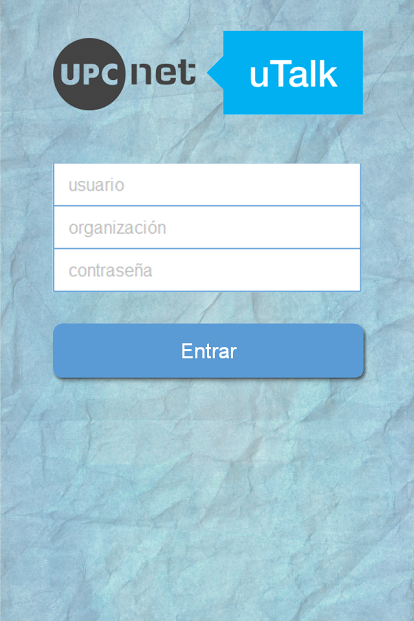
\includegraphics[scale=0.518]{Memoria/Arquitectura/Projecte/Presentacio/disseny_login.png}
    \end{minipage}%
    \hfill
    \begin{minipage}[t]{.48\textwidth}
        \centering
        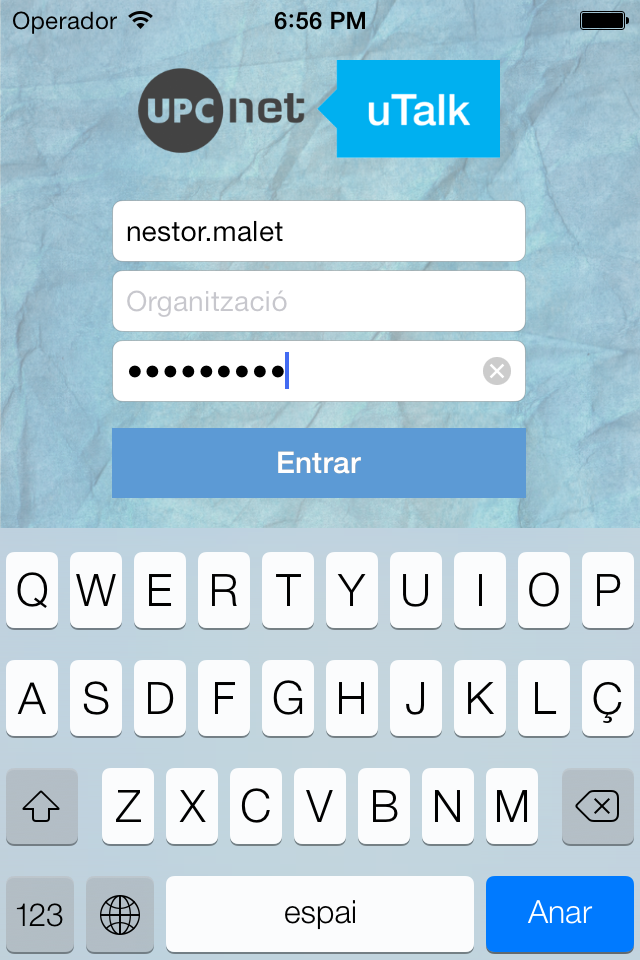
\includegraphics[scale=0.25]{Memoria/Implementacio/Captures/captura-login.png}
    \end{minipage}
    \caption{Comparació del disseny i el resultat de la vista}
    \label{fig:comparacio_disseny}
\end{figure}

Excepte a la vista d'inici de sessió, l'estructura del disseny extern segueix la mateixa estructura. A la figura \ref{fig:disseny_extern} es pot veure aquesta estructura amb els elements més importants marcats amb colors.

\begin{figure}[ht]
    \centering
    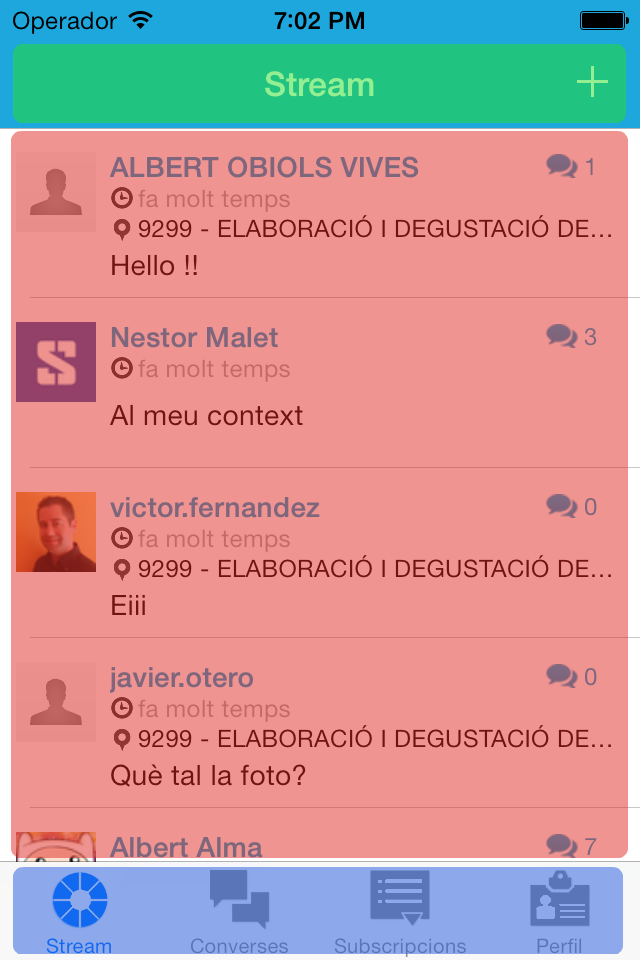
\includegraphics[scale=0.25]{Memoria/Arquitectura/Projecte/Presentacio/disseny_extern.png}
    \caption{Estructura del disseny extern del sistema}
    \label{fig:disseny_extern}
\end{figure}

L'element principal que organitza tot el sistema, són les pestanyes. A la figura aquest element està marcat amb color blau. Dintre de cada pestanya, la navegació es realitza mitjançant la barra de navegació, que a la figura està marcada amb color verd. I per acabar, al element de color vermell es mostra el contingut de cada vista.

\FloatBarrier